\section{Evaluation}
\label{sec:eval}

\iffalse
\begin{figure}[t]
\centering
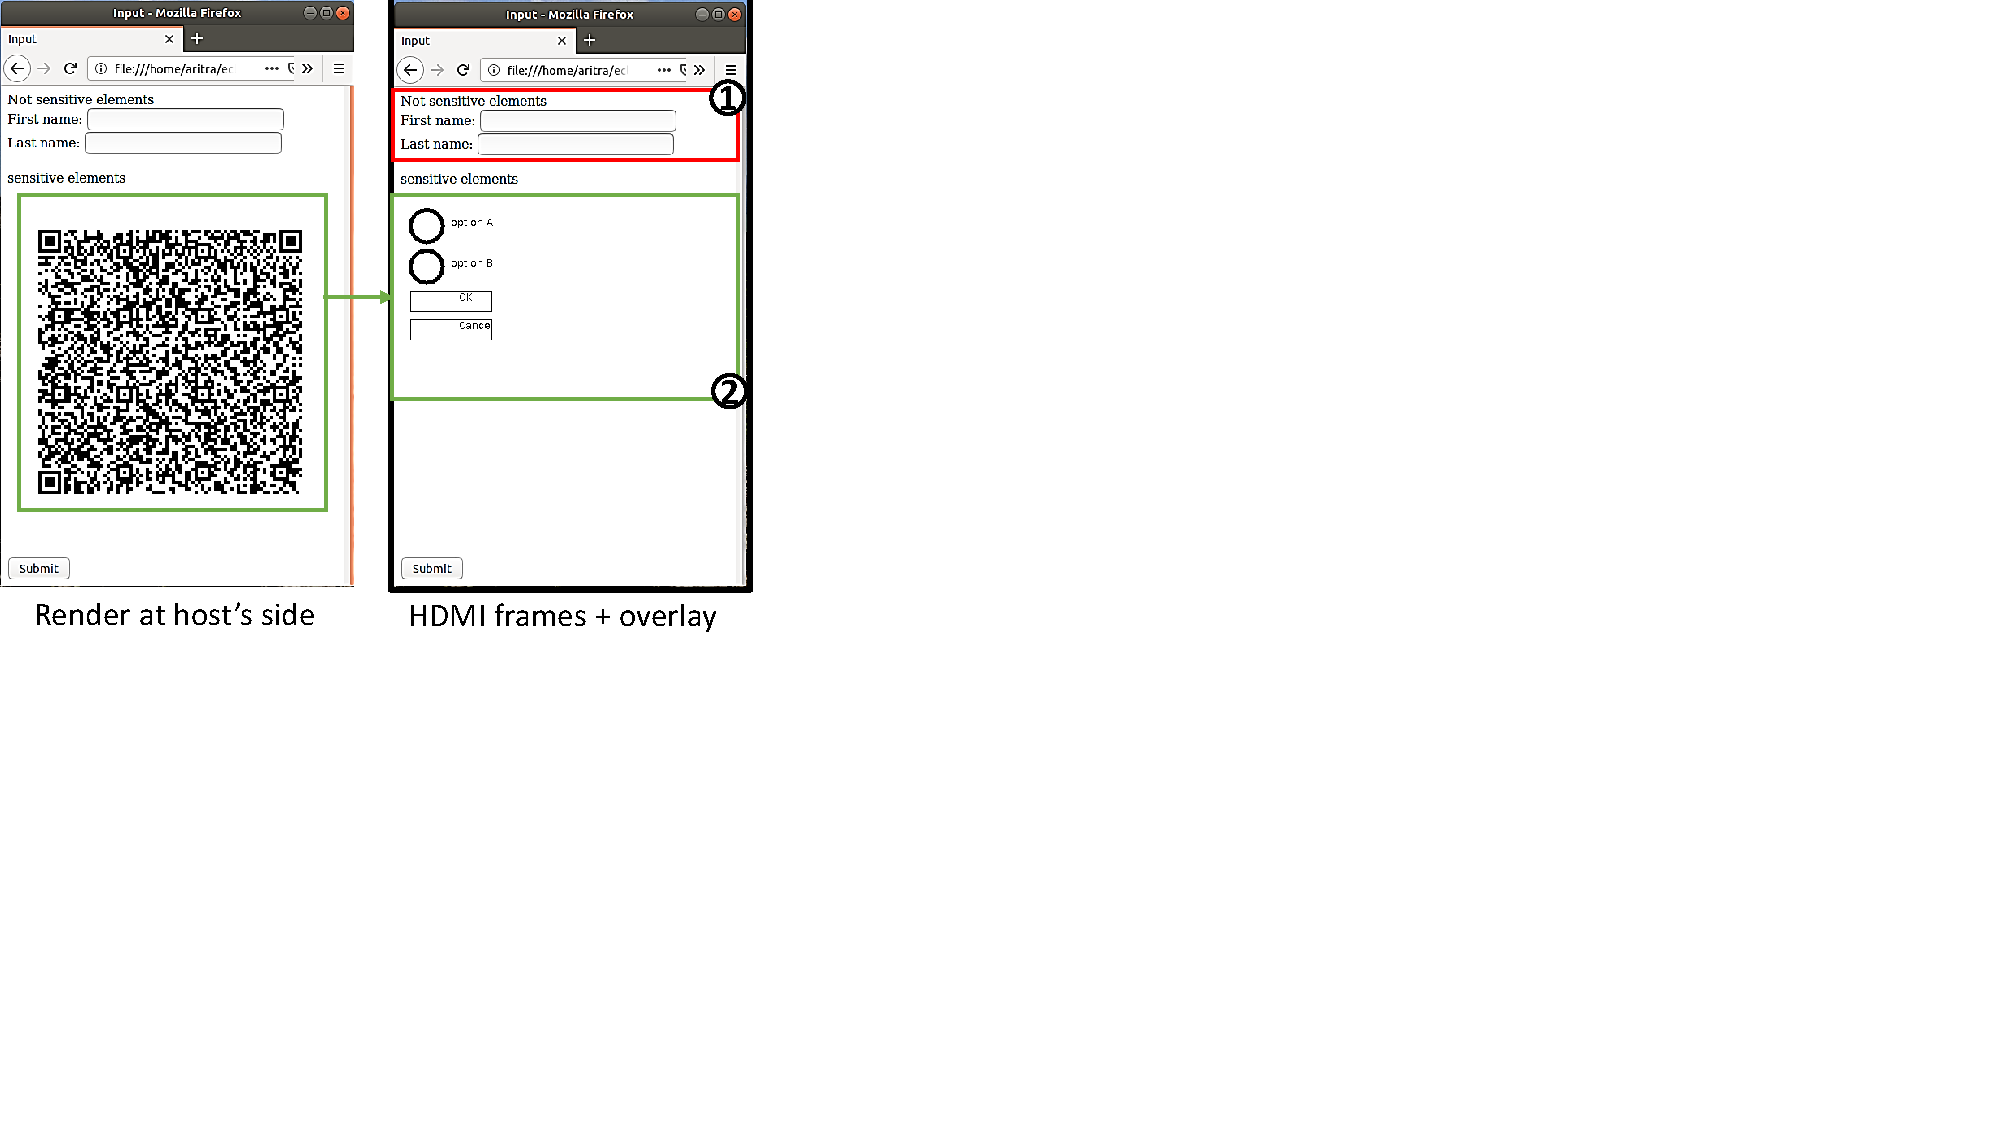
\includegraphics[trim={0 11cm 19cm 0}, clip, width=\linewidth]{overlayScreenShot.pdf}
\caption{\textbf{\name overlay}. }
\label{fig:screenshot_1}
\centering
\end{figure}
\fi


\begin{figure}[t]
\centering
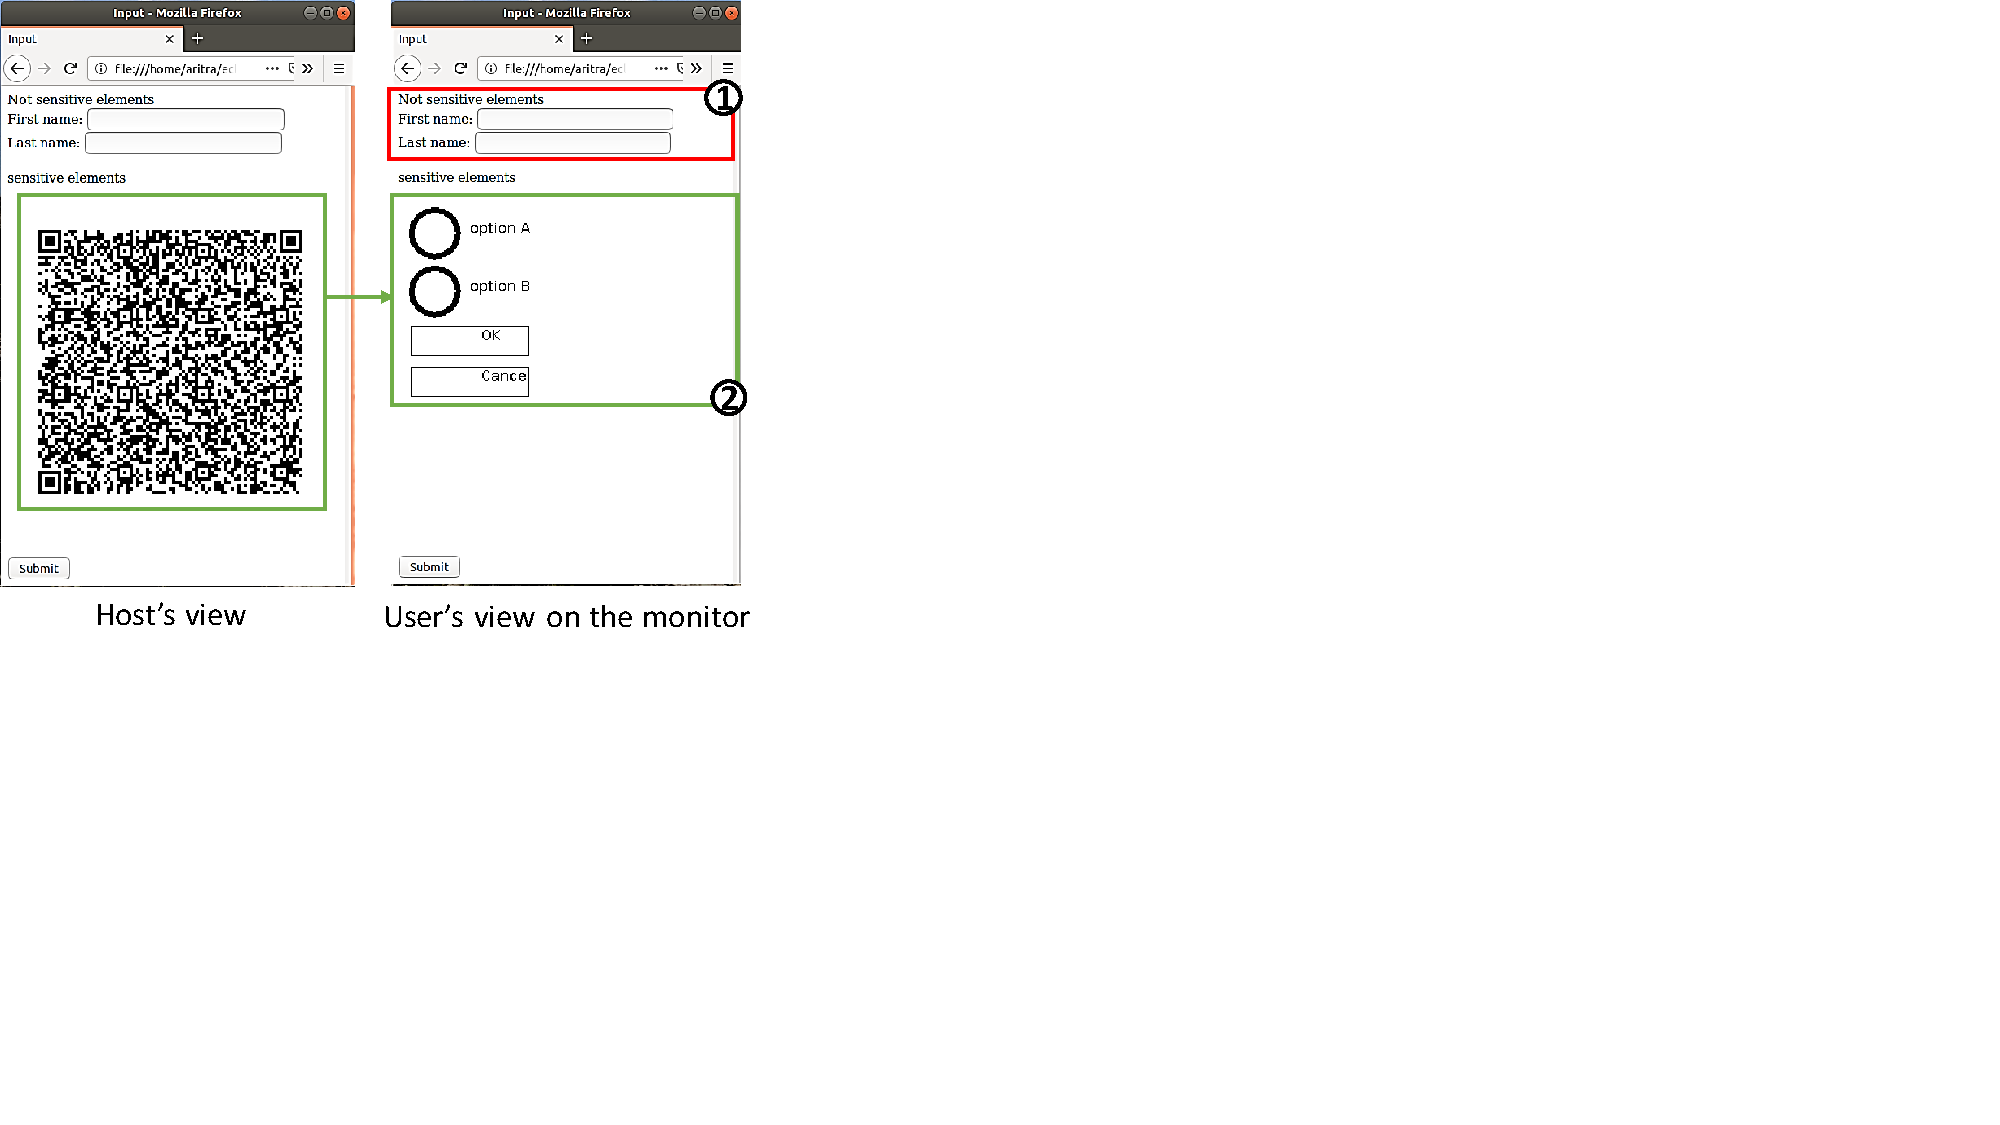
\includegraphics[trim={0 8cm 20cm 0}, clip, width=\linewidth]{overlayScreenShot_1.pdf}
\caption{\textbf{\device generated UI overlay} The figure shows the \name high-level approach. \one shows the non-protected part of the screen where the UI is rendered by the untrusted host. \two shows the \device generated protected UI overlay that is hidden from the host. The protected part of the screen provides integrity and confidentiality of all user IO.}
\spacesave
\label{fig:exampleImpelmentation}
\end{figure}


\begin{table}[t]
%\scriptsize
\centering
\begin{tabular}{l | c}
\textbf{Operation} & \textbf{Average time} \\\hline
Detecting mouse pointer & 1.76 ms \\
Detection QR code & 23 ms\\
Decoding QR code + Overlay & 6 ms\\
Mouse latency & 250 $\mu$s\\
Keyboard latency & 170 $\mu$s\\\hline
\end{tabular} 
\caption{Performance numbers}\spacesave
\end{table}

\subsection{Performance}

We evaluate the performance of our prototype by measuring the overheads introduced by \name to the system and whether they influence the user's interaction. Initially, we measure the default latency introduced by \device when the user interacts with applications that do not require protection. The delay to forward keystrokes is: \red{x ms} and frames is \red{x ms}. (This could be summarized in the end if numbers are very low.)

Our prototype of \name does not require the user to install any additional software in her machine in order to facilitate the communication between the remote server and the \device. Instead, the \device communicates with the remote server by using the host as an untrusted transporter. Therefore, we start by measuring the delay of sending data from the device to the host and vice versa:

\myparagraph{\device $\rightarrow$ host} The \device transmits data (encrypted) to the host by simulating keystrokes. In our system \device sends typical \red{x bytes} of data to the host. This takes \red{x ms}.

\myparagraph{Host $\rightarrow$ \device} The host sends data to the device by encoding them into the HDMI frame. The QR-code is generated locally in the browser and displayed on the screen. For a specification of a form with two/four elements QR-code generation takes \red{x ms}. The \device detects the QR-code, decodes it and creates the overlay. This process takes \red{x ms} for the same form considered previously.
 
For the applications that need protection \name introduces the following delays:

\myparagraph{Initial Page Load} First time the user visits a web page that employs \name, the remote server and the \device should exchange a cryptographic key to protect the communication. This step requires only \red{one additional ajax requst to the server} therefore the delay is relatively low. Initially, the browser encodes server's public key into a QR-code that is decoded by the \device, which sends the response to the server by simulating the keystrokes.

\myparagraph{Frame processing} \device processes every frame of the host. This takes \red{x ms} which hopefully is less than the frame rate.

\myparagraph{Keystroke latency} The \device intercepts all user's keystrokes and forwards them to the host or renders in the screen. When rendering on the screen, the latency is \red{x ms}.

\myparagraph{Cursor latency} Similarly to keystrokes, the \device intercepts mouse events also. However, the latency of event forwarding is \red{x ms}.


Key exchange takes around $200$ ms. Frame rate $20-24$ fps. Mouse/keyboard latency \textless$10ms$.